% Aula 03 - Matemática

\documentclass[a4paper]{article}
\usepackage[top=3cm,right=2cm,bottom=2cm,left=3cm]{geometry}
\usepackage[utf8]{inputenc}
\usepackage{amsmath}
\usepackage{graphicx} % imagens
\usepackage[portuguese]{babel} % ou brazil
% Ajusta hifenização, datas e nomes (como "Figura") para o português

\begin{document}
\begin{center}
    \textbf{Lista de Exercícios - 02}    
\end{center}

\begin{enumerate}

\item Calcule o determinante da seguinte matriz $A = 
\begin{bmatrix}
 4 & -4 \\
-6 & 16
\end{bmatrix}$.

\item Calcule a seguinte integral:
\[
\int_0^1 \left( x^3 + x^2 + x + \sqrt[5]{x+1} \right) \, dx
\]

\item Determine se a seguinte série é convergente.
\[
\sum_{k=1}^{\infty} \frac{1}{k^2}
\]

\end{enumerate}
\newpage

Imagem
\begin{figure}[h]
    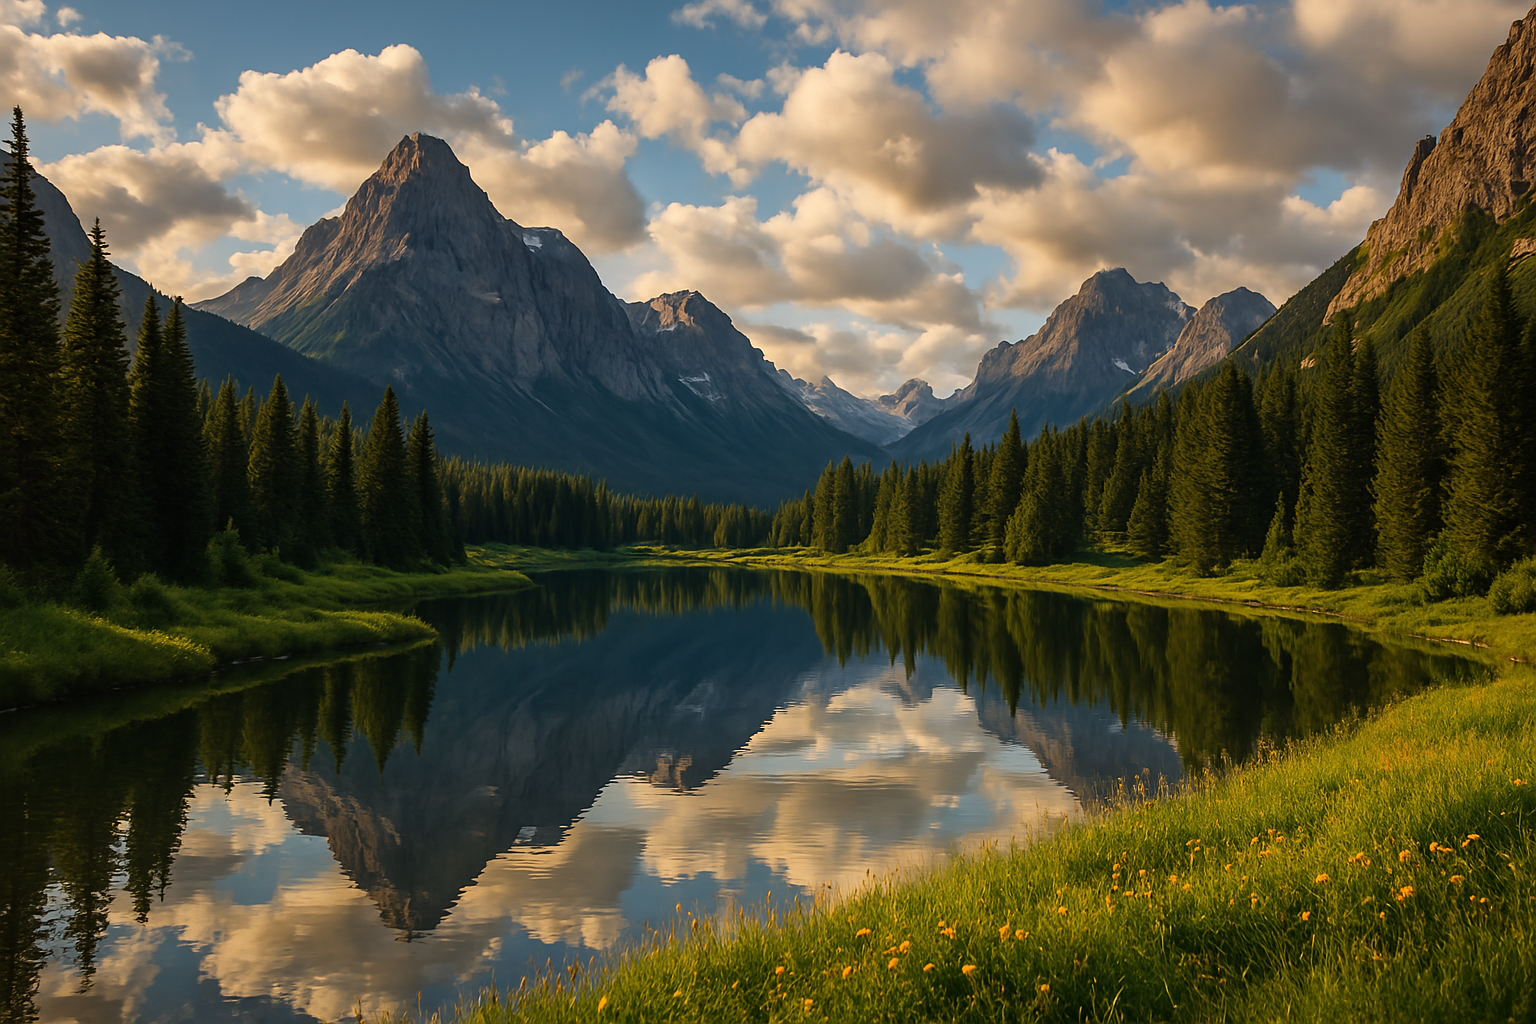
\includegraphics[angle=0, scale=0.15]{imagens/gpt.png}
\end{figure}

\newpage
\begin{center}
    \Large \bfseries Teste de figuras no \LaTeX
\end{center}
\begin{figure}[h]
    \centering
    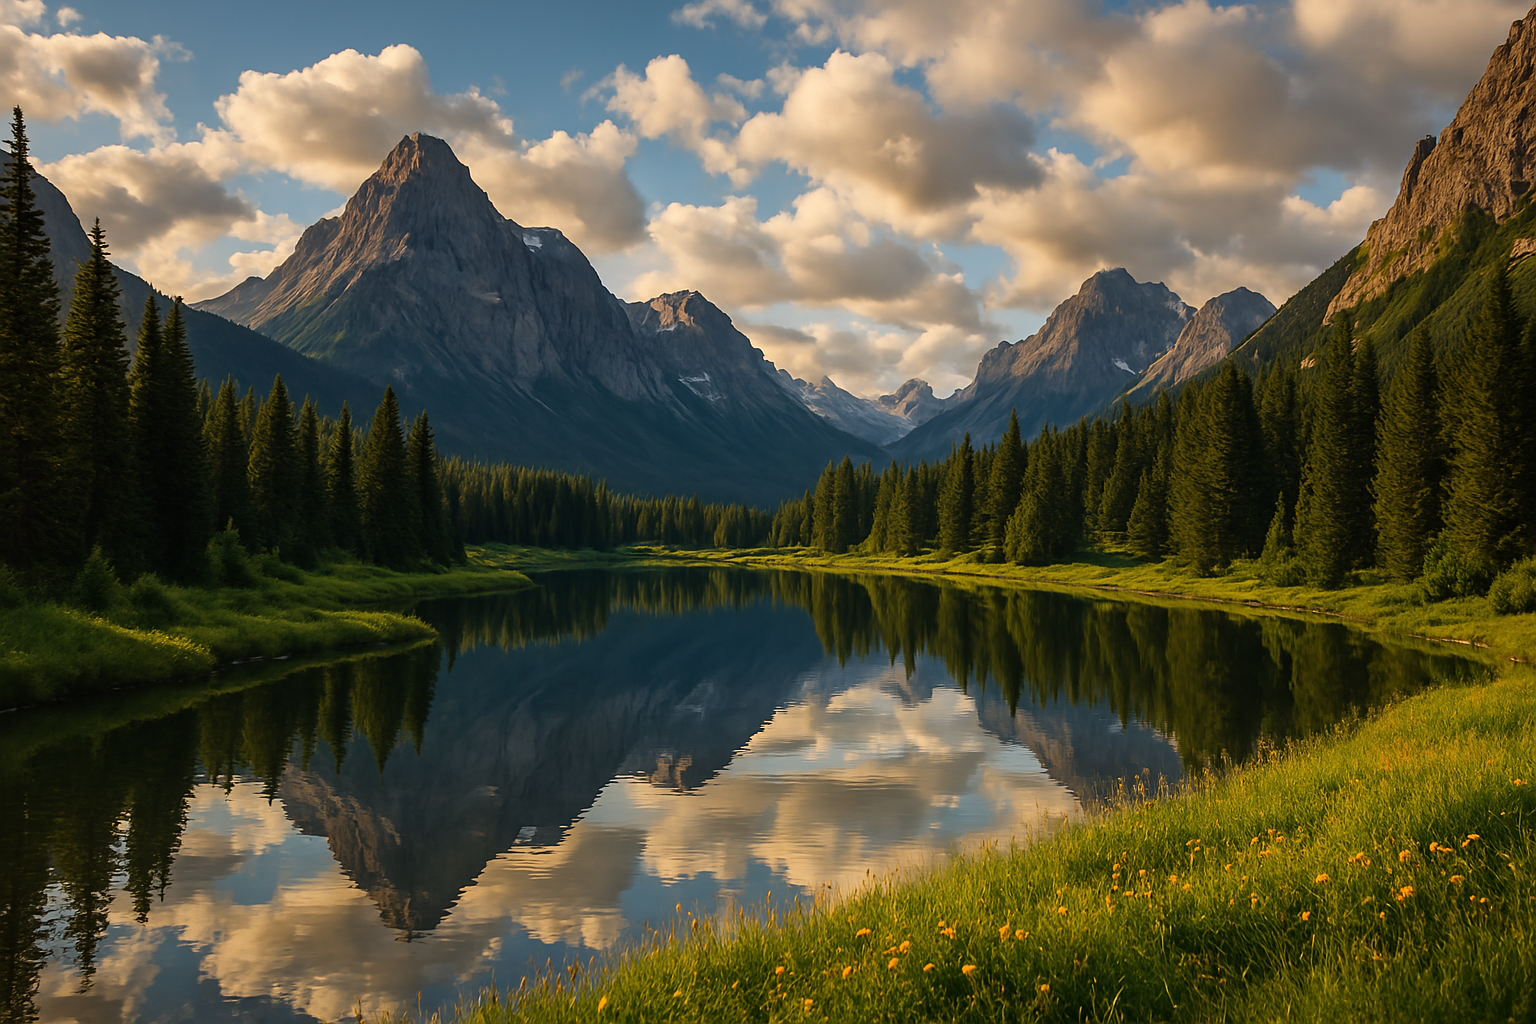
\includegraphics[angle=0, scale=0.1]{imagens/gpt.png}
    \caption{Sorria, pois você está aprendendo \LaTeX}
    \label{figura1}
\end{figure}

% Com o uso do {\bf label}, em qualquer lugar do texto você 
% pode fazer referência àquela figura, usando Figura \ref{figura1}
% para mencioná-la.

\newpage
\begin{figure}[htb]
\fbox{
    \begin{minipage}[b]{0.4\textwidth}
        \centering
            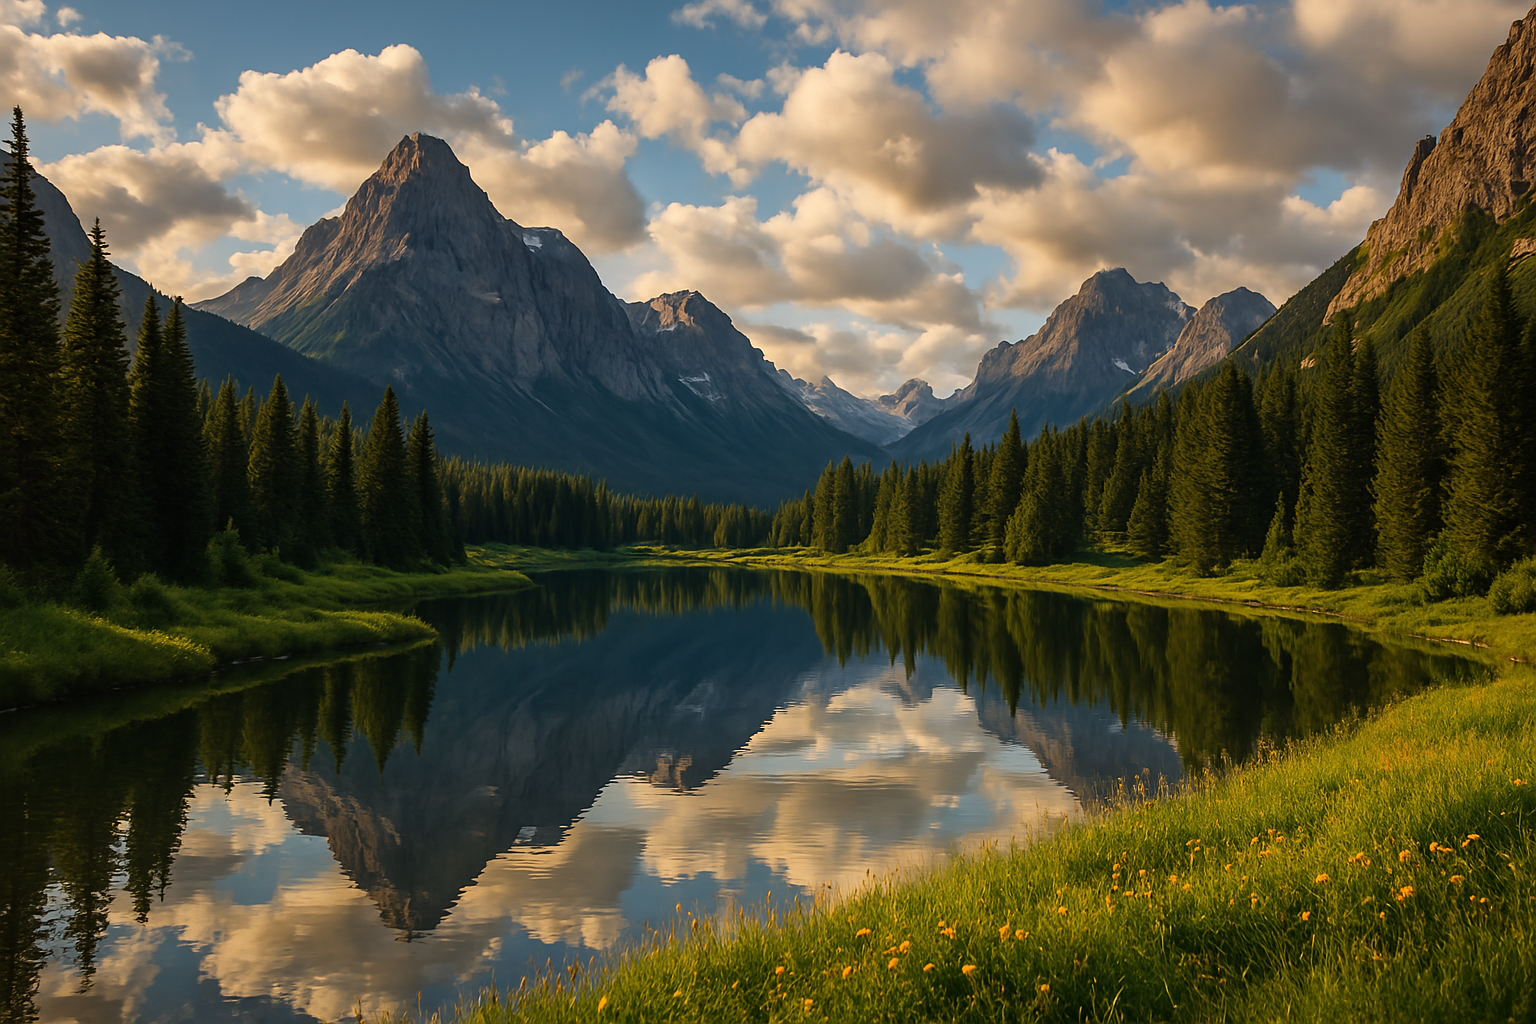
\includegraphics[width=0.5\textwidth]{imagens/gpt.png}
            \caption{Imagem com texto ao lado :)}
            \label{fig:by:text}
    \end{minipage}}
\fbox{
    \begin{minipage}[b]{0.4\textwidth}
        \centering
            Seu texto fica aqui!!!! :) \\
            Seu texto fica aqui!!!! :) \\
            Seu texto fica aqui!!!! :) \\
            Seu texto fica aqui!!!! :) \\
            Seu texto fica aqui!!!! :) \\
            Seu texto fica aqui!!!! :) \\
            Seu texto fica aqui!!!! :) \\
    \end{minipage}}
\end{figure}
\end{document}
